\documentclass[12pt]{article}
\usepackage{ArtigoIFPE}


\title{AVALIANDO O \textit{MERGE} SEMI-ESTRUTURADO: \\ um estudo comparativo de corretude e desempenho \\ da ferramenta SESAME}
\titleEng{EVALUATING SEMISTRUCTURED MERGE: a comparative evaluation of the SESAME tool}

\autora{David Lucas Alves de Almeida}
\emaila{dlaa@discente.ifpe.edu.br}
%\autorb{Nome do autor 2}
%\emailb{Email do autor 2}
% Aceita até 6 autores (autora, autorb, autorc, ... , autorf) e seus emails
\orientador{Guilherme José de Carvalho Cavalcanti}
\emailOrientador{guilherme.cavalcanti@belojardim.ifpe.edu.br}

\campus{Belo Jardim}
\curso{de Bacharelado em Engenharia de Software}
\data{18 de novembro de 2025}

\begin{document}

\maketitle

\thispagestyle{plain}

\section*{Resumo}

    \noindent A integração de modificações concorrentes é um desafio crítico no desenvolvimento colaborativo de software. Enquanto ferramentas de \textit{merge} não estruturadas (textuais) frequentemente geram conflitos espúrios, abordagens estruturadas, apesar de mais precisas, podem introduzir erros semânticos silenciosos e possuem alto custo computacional. Neste contexto, a ferramenta SESAME propõe uma abordagem semi-estruturada inovadora, utilizando separadores sintáticos para inferir a estrutura do código de forma leve. Este trabalho apresenta uma avaliação empírica do SESAME através de uma replicação diferenciada do estudo de Schesch et al. (2024). Adotando um protocolo experimental rigoroso, avaliou-se a ferramenta não apenas pela contagem de conflitos, mas pela corretude semântica verificada através da execução de suítes de testes automatizados em um vasto conjunto de projetos Java. O desempenho do SESAME foi contrastado com ferramentas do estado da arte (Git \textit{Merge}, Spork e IntelliMerge) utilizando um \textit{dataset} robusto com mais de 5.000 cenários de \textit{merge}, com métricas de Corretude, Tempo de Execução e Redução de Esforço (\textit{Effort Reduction}). Os resultados revelam que, embora ferramentas puramente estruturadas maximizem a resolução de conflitos, elas introduzem taxas elevadas de erros (11\% no Spork) e impõem latência proibitiva. Em contraste, o SESAME consolidou-se como um \textit{sweet spot}: manteve a segurança próxima ao padrão textual (apenas 3\% de erro) com um tempo de execução e uma ordem de grandeza inferior às ferramentas estruturadas, validando-se como uma alternativa pragmática e eficiente para esteiras de Integração Contínua.

\palavraschave{\textit{merge} Semi-Estruturado. Ferramentas de \textit{merge}. Conflitos de \textit{merge}. Avaliação de Desempenho. Corretude de Software.}

\section*{Abstract}

    \noindent The integration of concurrent modifications is a critical challenge in collaborative software development. While unstructured (textual) merge tools often generate spurious conflicts, structured approaches, although more accurate, can introduce silent semantic errors and have high computational costs. In this context, the SESAME tool proposes an innovative semi-structured approach, using syntactic separators to infer the code structure in a lightweight manner. This work presents an empirical evaluation of SESAME through a differentiated replication of the study by Schesch et al. (2024). Adopting a rigorous experimental protocol, the tool was evaluated not only by counting conflicts, but also by semantic correctness verified through the execution of automated test suites on a vast set of Java projects. SESAME's performance was compared with state-of-the-art tools (Git Merge, Spork, and IntelliMerge) using a robust dataset with over 5,000 merge scenarios, with metrics for Correctness, Execution Time, and Effort Reduction. The results reveal that, although purely structured tools maximize conflict resolution, they introduce high error rates (11\% in Spork) and impose prohibitive latency. In contrast, SESAME has established itself as a sweet spot: it maintained security close to the textual standard (only 3\% error) with an execution time and order of magnitude lower than structured tools, validating itself as a pragmatic and efficient alternative for Continuous Integration pipelines.

\keywords{Semistructured merge. Merge Tools. Merge Conflicts. Performance Evaluation. Merge Correctness.}

\vspace*{20pt} \hrule height 1.5pt

\section{Introdução}

    O desenvolvimento de software moderno é um processo inerentemente colaborativo, onde equipes trabalham simultaneamente em diferentes partes de um mesmo projeto. Para coordenar essas contribuições, Sistemas de Controle de Versão (VCS), como o Git, são indispensáveis. No entanto, a operação de \textit{merge}, que é o mecanismo central para integrar o trabalho de diferentes desenvolvedores, permanece um desafio crítico e um conhecido problema na engenharia de software.

    As ferramentas de \textit{merge} tradicionais, ditas não estruturadas (ou textuais), tratam o código como simples sequências de linhas. Embora sejam rápidas e universais, elas carecem de compreensão sintática, o que frequentemente resulta em ``conflitos espúrios'' em mudanças que são, na verdade, semanticamente independentes, conforme \textcite{cavalcanti2024semistructured}. No outro extremo, ferramentas estruturadas analisam a árvore sintática do código (AST) para evitar esses conflitos, mas à custa de maior complexidade e especificidade para cada linguagem. \parencite{schesch2024evaluation} Neste cenário, surge uma terceira via: o \textit{merge} semi-estruturado. Esta abordagem procura um equilíbrio, analisando estruturas de alto nível (como classes e métodos) e tratando o resto como texto. A ferramenta SESAME insere-se nesta categoria, propondo uma técnica inovadora que utiliza separadores sintáticos para refinar a resolução de conflitos sem a complexidade de uma análise sintática completa.
    
    Contudo, a eficácia destas ferramentas tem sido difícil de medir. Historicamente, a avaliação de ferramentas de \textit{merge} tem sido limitada por metodologias que não distinguem adequadamente um \textit{merge} correto de um incorreto. Como demonstrado no estudo recente de \textcite{schesch2024evaluation}, intitulado ``Evaluation of Version Control \textit{Merge} Tools'', muitos estudos anteriores focaram-se apenas na contagem de conflitos reportados. Esta métrica é enganadora: uma ferramenta pode ser ``silenciosa'' (não reportar conflitos), mas gerar um código com \textit{merge} incorreto, introduzindo erros de compilação ou bugs sutis no comportamento do programa. O autor argumenta que um \textit{merge} incorreto é significativamente mais custoso para o ciclo de desenvolvimento do que um conflito explícito, pois exige depuração posterior. Este trabalho propõe-se a preencher uma lacuna na literatura ao avaliar empiricamente a ferramenta SESAME sob uma ótica de rigor metodológico que faltou às suas avaliações preliminares.
    
    Para tal, este estudo configura-se como uma replicação diferenciada (\textit{differentiated replication}) do trabalho de \textcite{schesch2024evaluation}. A replicação de estudos experimentais é um pilar fundamental para o amadurecimento da engenharia de software como ciência, permitindo verificar a generalização de resultados e validar novas tecnologias em benchmarks estabelecidos. Enquanto o estudo original de \textcite{schesch2024evaluation} avaliou ferramentas como Git \textit{merge}, Spork e IntelliMerge, este trabalho estende a sua infraestrutura experimental para incluir e avaliar o SESAME. A avaliação não se baseará apenas na contagem de conflitos, mas utilizará a execução de suítes de testes automatizados em milhares de cenários de \textit{merge} reais (extraídos de projetos open-source) como um proxy para verificar a corretude do código resultante.

    O objetivo principal é determinar a eficácia do SESAME em termos de correção, desempenho e redução de esforço, posicionando-o comparativamente face ao estado da arte. Especificamente, este estudo pretende responder: onde se situa o SESAME no compromisso entre reduzir conflitos textuais e evitar a introdução de erros silenciosos.

\section{Fundamentação Teórica}
    Esta seção apresenta os conceitos fundamentais sobre controle de versão, as diferentes abordagens de \textit{merge} e as metodologias para avaliação da eficácia dessas abordagens. A operação de \textit{merge} é o processo pelo qual as contribuições de diferentes linhas de desenvolvimento são integradas.
    
    \subsection{Versionamento de Software e o Desafio do \textit{Merge}}
    O desenvolvimento de software moderno é uma atividade eminentemente colaborativa, na qual múltiplos desenvolvedores trabalham em paralelo. Para gerenciar essa complexidade, os Sistemas de Controle de Versão (VCS) são ferramentas indispensáveis. A operação de \textit{merge} é o processo pelo qual as contribuições de diferentes linhas de desenvolvimento são integradas. Os estudos de \textcite{Mens2002} sobre o tema mostram que o \textit{merge} de software é reconhecido como uma área de pesquisa complexa e desafiadora.

    O processo de \textit{merge} mais comum é o \textit{three-way merge} (\textit{merge} de três vias), que utiliza três versões de um arquivo para calcular o resultado final: a versão base (o ancestral comum mais próximo), e as duas versões modificadas, \textit{left} e \textit{right} (ou local e remota). O objetivo de uma ferramenta de \textit{merge} é integrar as alterações de forma automática. Quando isso não é possível, a ferramenta reporta um conflito, que exige intervenção manual do desenvolvedor.

    \subsection{O Espectro das Ferramentas de \textit{Merge}}
    As ferramentas de \textit{merge} podem ser classificadas em um espectro de abordagens, que variam em complexidade, precisão e custo computacional.

    \subsubsection{\textit{Merge} Não Estruturado (Textual)}
    A abordagem mais tradicional e amplamente utilizada, presente em ferramentas como o git \textit{merge} padrão, é o \textit{merge} não estruturado. Essa técnica trata os arquivos de código-fonte como simples sequências de linhas de texto, utilizando algoritmos como o diff3 para identificar e mesclar as diferenças \parencite{Khanna2007}.
    \begin{itemize}
    \item \textbf{Vantagens:} São rápidas, consomem poucos recursos e são agnósticas à linguagem de programação, podendo ser aplicadas a qualquer tipo de arquivo de texto.
    \item \textbf{Desvantagens:} Sua principal fraqueza é a falta de compreensão sobre a estrutura sintática do código. Isso leva à geração de conflitos espúrios (falsos positivos), por exemplo, quando dois desenvolvedores adicionam métodos diferentes na mesma região do arquivo. Além disso, podem falhar em detectar conflitos semânticos reais (falsos negativos), resultando em \textit{merges} que parecem limpos, mas que quebram a compilação ou o comportamento do programa.
    \end{itemize}

    \subsubsection{\textit{Merge} Estruturado}
    Para superar as limitações do \textit{merge} textual, pes\-qui\-sa\-do\-res de\-sen\-vol\-ve\-ram o \textit{mer\-ge} estruturado, que analisa a estrutura sintática do código-fonte. Ferramentas como o Spork baseiam-se em correspondência de nós em ASTs, enquanto o IntelliMerge  utiliza grafos de elementos de programa. Ambas buscam precisão máxima, mas sofrem com o \textit{overhead} de de\-sem\-pe\-nho e com\-ple\-xi\-da\-de de im\-ple\-men\-ta\-ção.
    \begin{itemize}
    \item \textbf{Vantagens:} Ao compreender a estrutura do programa, podem resolver conflitos que confundem as ferramentas textuais, como a reordenação de declarações de métodos ou campos. Isso resulta em uma maior precisão e na redução de conflitos espúrios.
    \item \textbf{Desvantagens:} São inerentemente específicas para cada linguagem, exigindo um esforço significativo de implementação para cada nova linguagem suportada. Além disso, as análises e \textit{merges} de ASTs completas podem ser computacionalmente caras, especialmente em arquivos grandes. Exemplos notáveis de ferramentas estruturadas incluem JDime, Spork e Mastery.
    \end{itemize}

    \subsubsection{\textit{Merge} Semi-Estruturado}
    Buscando um ponto de equilíbrio, a abordagem semi-estruturada foi proposta como um híbrido entre as duas anteriores. Ferramentas semi-estruturadas, como a FSTMerge, analisam apenas as estruturas de alto nível do código (como declarações de classes, métodos e campos), representando-as em uma AST parcial. As estruturas de baixo nível, como corpos de métodos e expressões, são tratadas como texto plano e mescladas com o auxílio de uma ferramenta não estruturada \parencite{Apel2011}.
    
    Embora essa abordagem reduza a com\-ple\-xi\-da\-de e o custo com\-pu\-ta\-cio\-nal do \textit{mer\-ge} es\-tru\-tu\-ra\-do, ela herda parte das im\-pre\-ci\-sões do \textit{mer\-ge} textual ao lidar com as es\-tru\-tu\-ras de baixo nível.

    \subsubsection{A Abordagem Inovadora do SESAME}
    Dentro da categoria semi-estruturada, a ferramenta SESAME, proposta por \textcite{cavalcanti2024semistructured}, introduz uma técnica inovadora. Em vez de se basear em uma AST parcial, a SESAME infere a estrutura do código alavancando separadores sintáticos específicos da linguagem (como {, }, (, ), ; em Java). A ferramenta pré-processa as versões do código, inserindo quebras de linha antes e depois de cada separador. Isso faz com que blocos de código que antes estavam na mesma linha (por exemplo, a condição e o corpo de um if) passem a ocupar linhas distintas e não-consecutivas. Em seguida, um algoritmo de \textit{merge} não estruturado é invocado sobre o código pré-processado, sendo capaz de resolver muitos conflitos que a abordagem semi-estruturada tradicional não conseguiria.
    
    Para ilustrar o funcionamento, considere o mecanismo de inferência de estrutura. Conforme detalhado por \textcite{cavalcanti2024semistructured}, o processo segue três etapas principais:
    \begin{itemize}
    \item \textbf{Pré-processamento:} A ferramenta insere quebras de linha e marcadores especiais (\textit{placeholders}) antes e depois de cada separador sintático. Isso isola os blocos lógicos em linhas distintas.
    \item \textbf{\textit{Merge} Textual:} Uma ferramenta não estruturada (diff3) é executada sobre esse código transformado. Como os blocos agora estão em linhas diferentes, o algoritmo textual consegue distinguir mudanças que antes colidiriam na mesma linha.
    \item \textbf{Pós-processamento}: Os marcadores e quebras de linha artificiais são removidos, restaurando o código original com o \textit{merge}.
    \end{itemize}
    
    \subsection{Exemplo Prático de Comportamento das Ferramentas}
    Para demonstrar a capacidade das ferramentas em resolver conflitos granulares, utiliza-se um cenário que envolve modificações simultâneas na definição de um laço de repetição (\textit{loop}) e a adição de novos métodos.

    A Figura \ref{fig:cenario_input} apresenta o estado inicial:
    \begin{itemize}
        \item \textbf{Base:} Método \texttt{iterar} padrão.
        \item \textbf{\textit{Left}:} Altera o início do laço (\texttt{i=1}) e adiciona o método \texttt{subtrair}.
        \item \textbf{\textit{Right}:} Altera o fim do laço (\texttt{i<11}) e adiciona o método \texttt{multiplicar}.
    \end{itemize}

    \begin{figure}[ht]
        \centering
        % Base
        \begin{minipage}{0.55\textwidth}
        \centering
            \textbf{Base}
            \begin{lstlisting}[language=Java, basicstyle=\ttfamily\scriptsize, frame=single, breaklines=true]
public class Teste {
    public void iterar() {
        for (int i = 0; i < 10; i++) {
            System.out.println("Iteração: " + i);
        }
    }
}
            \end{lstlisting}
        \end{minipage}
        \vspace{0.5cm}
        % Left
        \begin{minipage}{0.45\textwidth}
            \centering
            \textbf{\textit{Left} (Local)}
            \begin{lstlisting}[language=Java, basicstyle=\ttfamily\scriptsize, frame=single, breaklines=true]
public class Teste {
    public void iterar() {
        for (int i = 1; i < 10; i++) {
            System.out.println("Iteração: " + i);
        }
    }
    public int subtrair(int a, int b) {
        return a - b;
    }
}
            \end{lstlisting}
        \end{minipage}
        \hspace{0.5cm}
        % Right
        \begin{minipage}{0.45\textwidth}
            \centering
            \textbf{\textit{Right} (Remoto)}
            \begin{lstlisting}[language=Java, basicstyle=\ttfamily\scriptsize, frame=single, breaklines=true]
public class Teste {
    public void iterar() {
        for (int i = 0; i < 11; i++) {
            System.out.println("Iteração: " + i);
        }
    }
    public int multiplicar(int a, int b) {
        return a * b;
    }
}
            \end{lstlisting}
        \end{minipage}
        \caption{Cenário de \textit{merge}: modificações concorrentes na mesma linha do \texttt{for} e adição simultânea de métodos distintos.}
        \label{fig:cenario_input}
    \end{figure}

    A seguir, demonstra-se como cada categoria de ferramenta processa este cenário.

    \subsubsection{\textit{Merge} Textual (Git \textit{Merge})}
    O Git \textit{Merge} (não estruturado) trata o arquivo como uma sequência de linhas. Como existem modificações que ocorreram no mesmo ponto de inserção nos dois lados, a ferramenta não consegue determinar a ordem correta e reporta um conflito, exigindo intervenção manual (Figura \ref{fig:resultado_git}).

    \begin{figure}[ht]
    \centering
    \begin{minipage}{0.75\textwidth} % Aumentei a largura para caber tudo bem
        \centering
        \begin{lstlisting}[language=Java, basicstyle=\ttfamily\scriptsize, frame=single, keywordstyle=\color{blue}, breaklines=true, escapechar=!]
public class Teste {

    public void iterar() {
!\textcolor{red}{\textbf{<<<<<<< HEAD}}!
        for (int i = 1; i < 10; i++) {
!\textcolor{red}{\textbf{=======}}!
        for (int i = 0; i < 11; i++) {
!\textcolor{red}{\textbf{>>>>>>> branch-right}}!
            System.out.println("Iteração: " + i);
        }
    }

!\textcolor{red}{\textbf{<<<<<<< HEAD}}!
    public int subtrair(int a, int b) {
        return a - b;
    }
!\textcolor{red}{\textbf{=======}}!
    public int multiplicar(int a, int b) {
        return a * b;
    }
!\textcolor{red}{\textbf{>>>>>>> branch-right}}!
}
        \end{lstlisting}
    \end{minipage}
    \caption{Falha dupla do Git \textit{Merge}. Ocorre um conflito intra-linha na definição do laço \texttt{for} e um conflito de inserção no final da classe, onde a ferramenta não consegue determinar a ordem de inclusão dos novos métodos \texttt{subtrair} e \texttt{multiplicar}.}
    \label{fig:resultado_git}
    \end{figure}

    \subsubsection{\textit{Merge} Estruturado (Spork)}
    O Spork (es\-tru\-tu\-ra\-do) transcende a visão textual ao construir a Árvore Sintática Abstrata (AST). Ele identifica que as mo\-di\-fi\-ca\-ções no laço \texttt{for}, embora ocupem a mesma linha física, referem-se a nós filhos distintos dentro da estrutura do \texttt{For\-State\-ment}: a i\-ni\-ci\-a\-li\-za\-ção (\texttt{For\-Init}) alterada pelo ramo \textit{Left} e a expressão de condição (\texttt{Ex\-pres\-sion}) ajustada pelo ramo \textit{Right}.

    Além disso, ao analisar o escopo da classe \texttt{Teste}, a ferramenta interpreta as inserções ao final do arquivo não como uma colisão de blocos de texto, mas como a adição de dois novos nós \texttt{MethodDeclaration} independentes (\texttt{subtrair} e \texttt{multiplicar}). Isso permite que o Spork realize uma fusão granular das propriedades do laço e, simultaneamente, anexe os novos métodos como irmãos na árvore, resultando em um código válido e sem conflitos (Figura \ref{fig:ast_spork_result}).

    \subsubsection{\textit{Merge} Semi-estruturado (SESAME)}
    O SESAME (semi-estruturado) utiliza separadores sintáticos (‘\texttt{\{}’, ‘\texttt{\}}’, ‘,’, ‘(’, ‘)’ e ‘;’) para inferir a estrutura. Ao pré-processar o texto inserindo quebras de linha nos separadores, ele isola os blocos de código. Isso permite que o algoritmo textual subjacente distinga as duas inserções como blocos independentes, alcançando o mesmo resultado de sucesso do Spork, mas com menor custo computacional (Figura \ref{fig:resultado_spork_sesame}).

    \begin{figure}[H]
        \centering
        \begin{minipage}{0.75\textwidth}
            \centering
            \begin{lstlisting}[language=Java, basicstyle=\ttfamily\small, frame=single, keywordstyle=\color{blue}]
public class Teste {

    public void iterar() {
        for (int i = 1; i < 11; i++) {
            System.out.println("Iteração: " + i);
        }
    }

    public int subtrair(int a, int b) {
        return a - b;
    }

    public int multiplicar(int a, int b) {
        return a * b;
    }
    
}
            \end{lstlisting}
        \end{minipage}
        \caption{Resultado obtido tanto pelo Spork quanto pelo SESAME: fusão automática bem-sucedida (Clean \textit{merge}).}
        \label{fig:resultado_spork_sesame}
    \end{figure}

    \subsection{Visualização do Processamento Interno}

    Para compreender por que o resultado difere, é necessário observar a representação interna que cada ferramenta constrói a partir do código fonte.

    \subsubsection{Representação em Árvore (Estruturado)}
    Enquanto o Git opera cegamente sobre linhas de texto, o Spork converte o código em uma Árvore Sintática Abstrata (AST). A Figura \ref{fig:ast_spork_result} ilustra a hierarquia estrutural interpretada pela ferramenta. 

    O conflito é mitigado porque o Spork não enxerga uma colisão de caracteres na linha do laço, mas sim alterações em nós filhos distintos do \texttt{ForStatement}: a inicialização (\texttt{ForInit}) vinda do \textit{Left} e a condição de parada (\texttt{Expression}) vinda do \textit{Right}. Simultaneamente, a ferramenta compreende que os métodos \texttt{subtrair} e \texttt{multiplicar} são novos nós independentes que devem ser anexados ao nó pai \texttt{ClassDeclaration}, permitindo a reconciliação completa da estrutura.

    \begin{figure}[ht]
    \centering
    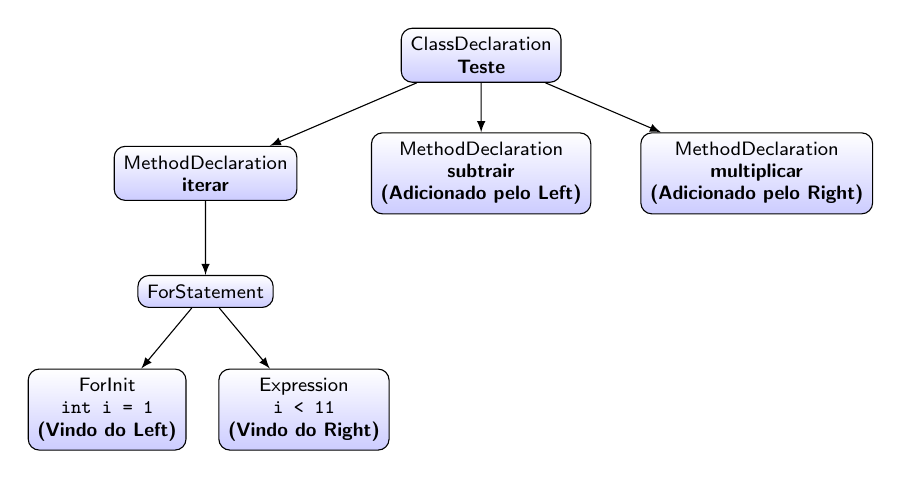
\begin{tikzpicture}[
        level distance=1.5cm,
        level 1/.style={sibling distance=3.5cm},
        level 2/.style={sibling distance=3cm},
        level 3/.style={sibling distance=2.5cm},
        every node/.style = {
            shape=rectangle, 
            rounded corners,
            draw, 
            align=center,
            font=\sffamily\scriptsize,
            top color=white, 
            bottom color=blue!20
        },
        edge from parent/.style={draw, -latex}
    ]
            
    % RAIZ
    \node {ClassDeclaration \\ \textbf{Teste}}
        % FILHO 1
        child { 
            node {MethodDeclaration \\ \textbf{iterar}} 
            child {
                node {ForStatement}
                child { node {ForInit \\ \texttt{int i = 1} \\ \textbf{(Vindo do \textit{Left})}} }
                child { node {Expression \\ \texttt{i < 11} \\ \textbf{(Vindo do \textit{Right})}} }
            }
        }
        % FILHO 2
        child { 
            node {MethodDeclaration \\ \textbf{subtrair} \\ \textbf{(Adicionado pelo \textit{Left})}} 
        }
        % FILHO 3
        child { 
            node {MethodDeclaration \\ \textbf{multiplicar} \\ \textbf{(Adicionado pelo \textit{Right})}} 
        };
    \end{tikzpicture}
    \caption{Árvore Sintática Abstrata (AST) resultante do Spork.}
    \label{fig:ast_spork_result}
    \end{figure}

    \subsubsection{Representação com Separadores (SESAME)}
    O SESAME não constrói a árvore completa, mas transforma o arquivo inserindo marcadores artificiais ao redor de separadores sintáticos específicos: \textbf{\{ \}, ( ), ; e ,} \parencite{cavalcanti2024semistructured}.

    A Figura \ref{fig:sesame_intermediate} demonstra como as linhas de código são ``explodidas'' verticalmente. Observe como os parênteses, vírgulas e pontos-e-vírgulas são isolados por marcadores \texttt{\$\$\$\$\$\$}. Isso permite que o algoritmo de \textit{diff} alinhe a estrutura do código mesmo se houver mudanças em linhas adjacentes.

    \begin{figure}[ht]
        \centering
        % Left
        \begin{minipage}{0.48\textwidth}
            \centering
            \textbf{\textit{Left} (Transformado)}
            % Usando \tiny para caber a "explosão" vertical do código
            \begin{lstlisting}[language=Java, basicstyle=\ttfamily\tiny, frame=single, backgroundcolor=\color{yellow!10}, showstringspaces=false, breaklines=true, keywordstyle=\color{blue}]
public class Teste 
$$$$$${
    public void iterar
    $$$$$$(
    $$$$$$) 
$$$$$${
        for 
        $$$$$$(
        $$$$$$int i = 1
        $$$$$$;
        $$$$$$i < 10
        $$$$$$; 
        $$$$$$i++
        $$$$$$) 
        $$$$$${
            System.out.println
            $$$$$$(
                $$$$$$"Iteração: " + i
            $$$$$$)
            $$$$$$;
        $$$$$$}
$$$$$$}
    public int subtrair
    $$$$$$(int a
    $$$$$$, 
    $$$$$$int b
    $$$$$$) 
    $$$$$${
        return a - b
        $$$$$$;
    $$$$$$}
$$$$$$}
            \end{lstlisting}
        \end{minipage}
        \hfill
        % Right
        \begin{minipage}{0.48\textwidth}
            \centering
            \textbf{\textit{Right} (Transformado)}
            \begin{lstlisting}[language=Java, basicstyle=\ttfamily\tiny, frame=single, backgroundcolor=\color{yellow!10}, showstringspaces=false, breaklines=true, keywordstyle=\color{blue}]
public class Teste 
$$$$$${
    public void iterar
    $$$$$$(
    $$$$$$) 
$$$$$${
        for 
        $$$$$$(
        $$$$$$int i = 0
        $$$$$$;
        $$$$$$i < 11
        $$$$$$; 
        $$$$$$i++
        $$$$$$) 
        $$$$$${
            System.out.println
            $$$$$$(
                $$$$$$"Iteração: " + i
            $$$$$$)
            $$$$$$;
        $$$$$$}
$$$$$$}
    public int multiplicar
    $$$$$$(int a
    $$$$$$, 
    $$$$$$int b
    $$$$$$) 
    $$$$$${
        return a * b
        $$$$$$;
    $$$$$$}
$$$$$$}
            \end{lstlisting}
        \end{minipage}
        \caption{Visualização detalhada do SESAME: inserção de quebras e marcadores (\texttt{\$\$\$}) nos separadores sintáticos configurados, isolando cada elemento estrutural.}
        \label{fig:sesame_intermediate}
    \end{figure}

    \FloatBarrier
    \subsection{O Desafio de Avaliar Ferramentas de \textit{Merge}}
    Tão importante quanto desenvolver novas ferramentas é a capacidade de avaliá-las de forma justa e realista. Enquanto o desenvolvimento do SESAME foca na eficiência da resolução de conflitos, a sua validação necessita de um critério de aceitação mais rigoroso do que a mera contagem de linhas. Adota-se, portanto, a perspectiva de \textcite{schesch2024evaluation}, que prioriza a integridade semântica do software resultante.
    
    Conforme apontado por \textcite{schesch2024evaluation}, a literatura anterior sofre com metodologias que apresentam falhas significativas, listadas a seguir:
    \begin{enumerate}
        \item \textbf{Falta de Distinção da Correção:} A maioria das avaliações existentes mede o sucesso de uma ferramenta apenas pela sua capacidade de produzir um \textit{merge} limpo (sem conflitos), tratando todos os \textit{merges} limpos como igualmente bem-sucedidos. No entanto, um \textit{merge} limpo pode ser incorreto, ou seja, pode introduzir um erro de compilação ou um defeito de comportamento que só será detectado posteriormente.
        \item \textbf{Dados Pouco Representativos:} Muitas avaliações utilizam cenários de \textit{merge} sintéticos ou coletados apenas da branch principal dos repositórios, o que não reflete a variedade e a complexidade dos \textit{merges} que ocorrem em branches de desenvolvimento, que são frequentemente deletadas após o a conclusão do processo.
        \item \textbf{``Verdade Fundamental'' Questionável:} Alguns estudos comparam o resultado da ferramenta com a versão final do código \textit{commitada} pelo desenvolvedor. Contudo, se o próprio desenvolvedor utilizou uma ferramenta de \textit{merge} imperfeita para gerar essa versão, o estudo pode acabar penalizando uma ferramenta mais correta.
    \end{enumerate}

    Para superar essas limitações, uma metodologia de avaliação mais rigorosa foi proposta. Ela se baseia na execução de suítes de teste automatizadas como um proxy para a verificação da correção do \textit{merge}. Assim, um \textit{merge} limpo é classificado como correto se todos os testes passarem, e incorreto se algum teste falhar. Adicionalmente, a metodologia introduz uma métrica de ``Redução de Esforço'', que leva em conta o custo relativo (k) de um \textit{merge} incorreto, partindo da premissa de que consertar um bug silencioso é significativamente mais caro do que resolver um conflito de \textit{merge} explícito.

    \subsection{Replicação na Engenharia de Software}
    A replicação é um componente essencial do método científico, permitindo que a comunidade verifique se resultados empíricos são consistentes e generalizáveis para além do contexto de um único estudo. Segundo \textcite{carver2014replications}, a replicação pode ser definida como a repetição deliberada de um estudo empírico com o objetivo de determinar se os resultados originais podem ser reproduzidos. Sem a replicação, observações isoladas podem ser fruto do acaso ou de condições específicas irreprodutíveis, impedindo a consolidação do conhecimento na área.

    Na Engenharia de Software, as replicações podem ser classificadas em diferentes tipos, dependendo do grau de fidelidade ao estudo original. \textcite{shull2008role} distinguem entre replicações exatas, onde se busca seguir os procedimentos originais o mais fielmente possível, e replicações conceituais, que buscam responder à mesma questão de pesquisa utilizando métodos diferentes . \textcite{mantyla2010rethinking} expandem essa visão, discutindo as replicações diferenciadas, onde variações deliberadas são introduzidas nas variáveis do experimento, como a alteração da população estudada ou das ferramentas avaliadas, para testar a robustez das teorias.

    Este trabalho classifica-se como uma replicação diferenciada do estudo conduzido por \textcite{schesch2024evaluation}. Adota-se, de forma rigorosa, a mesma infraestrutura experimental, bem como as mesmas métricas de avaliação (correção via suítes de teste) e critérios de sucesso do estudo original. A diferenciação principal reside na introdução de uma nova variável independente: a ferramenta de \textit{merge} SESAME. Desta forma, o estudo não apenas valida a metodologia proposta por \textcite{schesch2024evaluation}, mas também estende o corpo de conhecimento ao avaliar o comportamento de uma nova abordagem semi-estruturada frente aos \textit{baselines} da literatura.

    \subsection{Síntese e Lacuna na Literatura}
    A literatura apresenta um campo de pesquisa ativo, com um espectro de ferramentas de \textit{merge} que buscam equilibrar simplicidade, desempenho e precisão. Ao mesmo tempo, emerge um consenso sobre a necessidade de metodologias de avaliação mais robustas, que considerem a correção do código resultante como a principal métrica de sucesso.
    
    Neste ponto, identifica-se uma clara lacuna: a ferramenta inovadora \textbf{SESAME}, com sua abordagem única baseada em separadores sintáticos, foi avaliada em seu trabalho original  antes da consolidação desta metodologia de avaliação mais sofisticada. Portanto, seu desempenho em termos de correção, sua taxa de geração de \textit{merges} incorretos e sua posição em comparação com o estado da arte (ferramentas como Spork, IVn, etc.) sob esta ótica mais rigorosa, são desconhecidas. 
    Este trabalho preenche essa lacuna ao executar o protocolo de \textcite{schesch2024evaluation} sobre o SESAME, permitindo uma comparação direta de \textit{Effort Reduction} com as ferramentas estado da arte.

\section{Metodologia}
    \subsection{Desenho do Estudo}
    Este estudo caracteriza-se como uma pesquisa experimental quantitativa. O desenho experimental segue o protocolo de replicação diferenciada, reutilizando a infraestrutura de avaliação, o conjunto de dados e as métricas propostas por \textcite{schesch2024evaluation}. A variável independente introduzida é a ferramenta de \textit{merge} SESAME, cujo desempenho será contrastado com as ferramentas de referência (\textit{baselines}) do estudo original: Git \textit{Merge} (abordagem textual) e Spork (abordagem estruturada).
    
    \subsection{Seleção e Preparação do Conjunto de Dados}
    Para garantir a representatividade dos resultados, utiliza-se o conjunto de dados curado por \textcite{schesch2024evaluation}, derivado de repositórios Java de alta qualidade listados nos \textit{datasets} ``\textit{GitHub's Greatest Hits}'' e ``\textit{Reaper}''.

    O processo de filtragem dos cenários de \textit{merge} obedeceu aos seguintes critérios rigorosos para isolar a responsabilidade da ferramenta:
    \begin{enumerate}
        \item \textbf{Relevância:} Apenas projetos Java que utilizam sistemas de automação de \textit{build} Maven ou Gradle.
        \item \textbf{Sanidade dos Pais:} Foram selecionados apenas cenários onde ambos os \textit{commits} pais (as duas versões a sofrerem o \textit{merge}) compilam e passam em todos os testes existentes. Isso assegura que qualquer falha detectada após o \textit{merge} foi causada exclusivamente pelo processo de \textit{merge} e não por defeitos pré-existentes.
        \item \textbf{Diversidade de Fontes:} O \textit{dataset} inclui tanto \textit{merges} do ramo principal (main branch) quanto de ramos secundários (\textit{feature branches}), capturando a complexidade real do fluxo de desenvolvimento, conforme recomendado por \textcite{schesch2024evaluation}.
    \end{enumerate}

    \subsection{Integração da Ferramenta SESAME}
    A infraestrutura original de Schesch foi projetada para ser extensível, exigindo que novas ferramentas sejam integradas via shell \textit{scripts} padronizados. Para permitir a avaliação do SESAME, foram desenvolvidos dois artefatos de integração distintos, seguindo as diretrizes do \textit{framework} original:
    \begin{enumerate}
        \item \textbf{Integração Básica (sesame.sh):} Foi desenvolvido um \textit{script wrapper} que configura o SESAME como um \textit{merge} driver nativo do Git. A implementação completa deste \textit{script} encontra-se no \textbf{Apêndice \ref{apendice:sesame_sh}}. Ele automatiza a invocação do executável sesame.jar utilizando a estratégia de separadores (-tms csdiff), garantindo que os parâmetros de revisão base, local e remota sejam passados corretamente.
        \item \textbf{Integração Híbrida (sesame\_plus.sh):} Para uma comparação justa com os resultados de \textcite{schesch2024evaluation}, que avaliaram ferramentas em conjunto com utilitários de limpeza, foi criado um segundo \textit{script} denominado \textit{sesame\_plus.sh} (disponível no \textbf{Apêndice \ref{apendice:sesame_plus}}). Este artefato orquestra a execução sequencial do SESAME seguida pela ferramenta Plume-lib \textit{Merging}, reutilizando a lógica de integração da infraestrutura original para garantir consistência com os \textit{baselines}.
    \end{enumerate}

    \subsection{Procedimento Experimental e Execução de Testes}
    A execução do experimento seguiu a infraestrutura de orquestração disponibilizada pelo estudo original. O processo não se resume a uma única etapa de processamento, mas constitui um fluxo de trabalho composto por sete estágios sequenciais. Esse \textit{pipeline} foi mantido integralmente nesta replicação para assegurar a comparabilidade dos dados, o isolamento de falhas e a fidelidade à metodologia de referência. Abaixo, descreve-se o fluxo de dados e os módulos de \textit{script} responsáveis por cada fase:

    \begin{enumerate}
        \item \textbf{Inicialização e Rastreabilidade}:
        A etapa inicial congela o estado dos repositórios analisados. O \textit{script} registra os \textit{hashes} exatos dos \textit{commits} (HEADs) de cada projeto no momento da execução. Esse procedimento assegura a rastreabilidade total do experimento, garantindo que qualquer tentativa futura de replicação utilize exatamente as mesmas versões do código-fonte, eliminando divergências causadas por atualizações nos repositórios remotos.

        \item \textbf{Validação de Sanidade}:
        Para mitigar ameaças à validade interna, o \textit{pipeline} realiza uma pré-validação dos pais do \textit{merge}. Antes de tentar qualquer fusão, o sistema executa a suíte de testes nos \textit{commits} originais (\textit{Left} e \textit{Right}). Apenas os cenários onde os pais passam nos testes (\textit{Tests\_passed}) são mantidos. Repositórios instáveis ou com falhas pré-existentes são descartados nesta etapa, garantindo que falhas observadas posteriormente sejam causadas exclusivamente pelo processo de \textit{merge} e não por defeitos anteriores.

        \item \textbf{Mineração e Amostragem}:
        O componente Java \texttt{FindMergeCommits} varre o histórico do Git para identificar cenários de \textit{merge} candidatos. Na sequência, o módulo de amostragem aplica critérios de filtragem rigorosos (como a exclusão de \textit{merges} triviais ou sem alterações de código). Com base no parâmetro de configuração $n\_merges$, o sistema seleciona a amostra final — seja o \textit{dataset} completo ou um subconjunto estatisticamente representativo.

        \item \textbf{Análise Estática Prévia}:
        Antes da execução das ferramentas, realiza-se uma caracterização dos cenários selecionados. Este módulo coleta métricas sobre a complexidade dos conflitos, número de arquivos envolvidos e linhas de código impactadas, preparando o terreno para correlacionar essas características com o sucesso ou falha das ferramentas posteriormente.

        \item \textbf{Execução e Teste de Corretude}:
        Este é o núcleo do processamento experimental. O \textit{script} itera sobre cada cenário de \textit{merge}, isola o ambiente e invoca a ferramenta alvo (SESAME, Spork ou Git, por exemplo). Após a tentativa de fusão, o sistema tenta compilar e executar a bateria de testes do projeto resultante. O estado final é capturado e classificado em categorias discretas: Sucesso, Falha de Compilação, Falha de Teste ou Conflito Não Resolvido.

        \item \textbf{Medição de Desempenho}:
        Executada sobre o \textit{dataset} de controle, esta etapa foca na coleta de métricas temporais. O \textit{pipeline} reexecuta os \textit{merges} instrumentando tanto o tempo de CPU quanto o tempo total (\textit{wall-clock}). Para assegurar precisão estatística e mitigar ruídos causados pelo ``aquecimento'' da JVM (\textit{warm-up}) ou \textit{cache} de disco, cada cenário é executado múltiplas vezes, calculando-se a média aritmética dos tempos válidos.

        \item \textbf{Consolidação de Resultados}:
        A etapa final agrega os \textit{logs} brutos e arquivos CSV gerados por todas as fases anteriores. O módulo processa estatisticamente os dados, calculando taxas de acerto (\textit{Recall}) e médias de tempo, e gera automaticamente os artefatos visuais (tabelas e gráficos em formato \LaTeX/PGF) apresentados neste trabalho, eliminando erros de transcrição manual.
    \end{enumerate}

    Essa abordagem em estágios garante que a avaliação dos algoritmos de \textit{merge} ocorra sobre dados limpos e verificados, isolando variáveis de confusão e assegurando a robustez das conclusões apresentadas.

    \subsubsection{Protocolo de Invocação das Ferramentas}
    Para cada cenário de \textit{merge} processado pelo estágio de execução (passo 5 acima), o protocolo de invocação das variantes (SESAME e SESAME+) obedece a um fluxo rigoroso de verificação:
    \begin{enumerate}
        \item \textbf{\textit{Checkout} e Preparação:} O \textit{framework} realiza o \textit{checkout} forçado da versão local (\textit{branch1}) e configura o estilo de conflito do Git para \texttt{diff3}, garantindo que os marcadores de conflito contenham a informação do ancestral comum.
        \item \textbf{Execução do \textit{Merge}:} O \textit{script wrapper} cor\-res\-pon\-den\-te (\texttt{se\-sa\-me.sh} ou \texttt{se\-sa\-me\_plus.sh}) é invocado. No caso do \textbf{SESAME+}, implementou-se uma lógica de contingência: se o SESAME padrão deixar conflitos não resolvidos, a biblioteca \textit{Plume-lib} é acionada imediatamente com a estratégia \texttt{merge-plumelib} na tentativa de resolver as seções restantes automaticamente.
        \item \textbf{Verificação de Sucesso:} O sistema verifica o código de retorno da ferramenta. Se for diferente de 0 ou se o Git ainda reportar arquivos com marcadores de conflito (\texttt{diff-filter=U}), o \textit{merge} é classificado como \textbf{Não Tratado (\textit{Unhandled})}.
        \item \textbf{Validação de Corretude:} Apenas se o \textit{merge} for reportado como limpo (código de retorno 0), o fluxo avança para a fase de compilação e execução da suíte de testes.
    \end{enumerate}

    \subsection{Métricas de Avaliação}
    A classificação dos resultados baseia-se na integridade semântica do código, e não apenas na textual:
    \begin{itemize}
        \item \textbf{\textit{Merge} Correto (\textit{Correct}):} \textit{Merge} limpo e todos os testes passam.
        \item \textbf{\textit{Merge} Incorreto (\textit{Incorrect}):} \textit{Merge} limpo, mas ocorre falha na compilação ou nos testes.
        \item \textbf{\textit{Merge} Não Tratado (\textit{Unhandled}):} A ferramenta reporta conflito.
    \end{itemize}
    
    \textbf{Métrica de Redução de Esforço (\textit{Effort Reduction}):} Para comparar quantitativamente as ferramentas, utiliza-se a métrica de \textit{Effort Reduction} proposta por \textcite{schesch2024evaluation}. Esta métrica penaliza desproporcionalmente os \textit{merges} incorretos, assumindo que corrigir um erro silencioso é mais custoso do que resolver um conflito explícito.
    
    A fórmula utilizada é:
    \begin{equation}
        Effort Reduction= 1 - \frac{Unhandled + (Incorrect \times k)}{NumMerges}
    \end{equation}
    Onde:
    \begin{itemize}
        \item \textit{k} é o fator de custo relativo de um \textit{merge} incorreto. Conforme a análise de sensibilidade de Schesch, o valor de \textit{k} varia (e.g., de 1 a 20) para demonstrar como a penalidade afeta o ranking das ferramentas.
    \end{itemize}

    \subsection{Disponibilidade de Dados e Materiais}
    A fim de garantir a transparência e a reprodutibilidade deste estudo, todo o código-fonte, \textit{scripts} de orquestração e os dados brutos gerados durante os experimentos foram disponibilizados publicamente.
    
    É importante ressaltar que, embora este documento discuta os resultados focados nas ferramentas \textbf{SESAME, Spork, IntelliMerge e Git \textit{Merge}} para fins de síntese e foco analítico, o repositório contém a execução estendida englobando todas as ferramentas avaliadas na infraestrutura original.

    \textbf{Nota sobre Execução Reduzida:} Adicionalmente, disponibiliza-se no mesmo repositório um \textit{dataset} de ``Execução Rápida'' (\textit{Shortcut}), contendo métricas coletadas sobre uma amostragem de 10 repositórios distintos (totalizando 100 \textit{commits} de \textit{merge}). Este subconjunto serve como referência para pesquisadores que desejam validar o ambiente de execução rapidamente sem a necessidade de processar a carga de trabalho massiva completa.

    O pacote de replicação completo encontra-se referenciado sob o identificador de \textcite{almeida2025repository} e pode ser acessado diretamente através do endereço:

    \begin{center} \url{https://github.com/davidalmd/AST-Merging-Evaluation-TCC} \end{center}
    
\section{Resultados}
    Nesta sessão, apresentam-se os dados obtidos a partir da execução experimental da ferramenta SESAME, contrastados com as ferramentas de referência (\textit{baselines}) definidas no estudo original de \textcite{schesch2024evaluation} e o estado da arte em \textit{merge} estruturado.

    \subsection{Visão Geral dos Dados de Corretude}

    A Tabela \ref{tab:resultados_gerais} sumariza o desempenho bruto de cada ferramenta sobre o conjunto de dados processados. A partir de um universo inicial de 69.119 candidatos minerados, aplicaram-se filtros de relevância (arquivos Java modificados) e sanidade (pais aprovados nos testes), resultando em um \textit{dataset} final composto por \textbf{5.365} cenários de \textit{merge} amostrados para execução.
    Observa-se que o \textit{dataset} desafiou significativamente todas as abordagens, com nenhuma ferramenta atingindo 60\% de taxa de sucesso sem intervenção manual.

    \begin{table}[ht]
    \centering
    \caption{Desempenho comparativo das ferramentas de \textit{merge}. Dados extraídos da execução experimental. Os valores indicam o número absoluto e a porcentagem em relação ao total de cenários.}
    \label{tab:resultados_gerais}
    \resizebox{\textwidth}{!}{% Ajusta a tabela à largura da página
        \begin{tabular}{|l|cc|cc|cc|}
            \hline
            \textbf{Ferramenta} & \multicolumn{2}{c|}{\textbf{Corretos}} & \multicolumn{2}{c|}{\textbf{Incorretos}} & \multicolumn{2}{c|}{\textbf{Não Tratados (Conflitos)}} \\
            & \# & \% & \# & \% & \# & \% \\ \hline
            Git \textit{Merge} (ort) & 2450 & 47\% & 92 & 2\% & 2682 & 51\% \\ \hline 
            Spork & 2889 & 55\% & 558 & 11\% & 1777 & 34\% \\ \hline 
            IntelliMerge & 446 & 9\% & 3659 & 70\% & 1119 & 21\% \\ \hline 
            \textbf{SESAME} & \textbf{2461} & \textbf{47\%} & \textbf{174} & \textbf{3\%} & \textbf{2589} & \textbf{50\%} \\ \hline 
            \textbf{SESAME+} & \textbf{2472} & \textbf{47\%} & \textbf{173} & \textbf{3\%} & \textbf{2579} & \textbf{49\%} \\ \hline
        \end{tabular}
    }
    \end{table}

    \subsection{Análise de Redução de Conflitos}
    A capacidade de resolver conflitos automaticamente varia drasticamente entre os paradigmas. O Git \textit{Merge} (ort) falhou em resolver \textbf{51\%} dos cenários (2682 casos).

    As ferramentas puramente estruturadas, como o Spork, demonstraram a maior agressividade na resolução, reduzindo a taxa de conflitos não tratados para \textbf{34\%}. Contudo, essa agressividade tem um custo na corretude, conforme discutido a seguir.

    O SESAME, posicionando-se como uma abordagem semi-estruturada, obteve uma taxa de conflitos não tratados de \textbf{50\%} (2589 casos). Embora a redução numérica direta em relação ao Git seja modesta (aproximadamente 3,5\% de redução no número absoluto de conflitos), o SESAME mantém a segurança próxima à do paradigma textual, evitando as distorções estruturais observadas em ferramentas mais complexas.

    \subsection{Análise de Corretude e Erros Silenciosos}
    A métrica mais crítica para a adoção industrial, como destacado por \textcite{schesch2024evaluation}, é a taxa de \textit{merges} incorretos — cenários onde a ferramenta reporta sucesso, mas o código resultante quebra (falha de compilação ou teste).

    \begin{itemize} 
        \item \textbf{O Risco Estruturado:} O Spork, apesar de resolver mais conflitos, introduziu erros em \textbf{11\%} dos casos (558 falhas). O IntelliMerge mostrou-se inviável para este \textit{dataset}, com uma taxa de erro de \textbf{70\%}, comportando-se como um \textit{outlier} negativo. 
        \item \textbf{A Segurança Semi-Estruturada:} O SESAME apresentou uma taxa de erro de apenas \textbf{3\%} (174 casos), um valor muito próximo ao do Git (2\%). 
    \end{itemize}

    Isso indica que o SESAME consegue aplicar inteligência estrutural (via separadores) sem assumir os riscos de ``alucinação estrutural'' que ferramentas baseadas em AST completa (como o Spork) tendem a cometer quando a árvore sintática não pode ser perfeitamente reconciliada.

    \subsection{Redução de Esforço (\textit{Effort Reduction})}
    Para ponderar o compromisso entre resolver conflitos e evitar erros, a métrica de \textit{Effort Reduction} penaliza as ferramentas conforme o custo k de corrigir um erro introduzido aumenta.
    
    A Figura \ref{fig:effort_reduction} (baseada no arquivo \texttt{cost\_without\_manual.pdf} gerado pelo experimento) ilustra este cenário:

    \begin{figure}[H]
        \centering
        \includegraphics[width=0.75\textwidth]{imagens/cost_without_manual.pdf}
        \caption{Curva de Redução de Esforço (\textit{Effort Reduction}). O eixo X representa o fator de custo k para erros incorretos. Fonte: Dados experimentais.}
        \label{fig:effort_reduction}
    \end{figure}

    Observa-se que:
    \begin{itemize}
        \item Para k=0 (custo de corrigir erro igual ao de resolver conflito), o Spork lidera devido à sua alta taxa de resolução bruta. 
        \item No entanto, a curva do Spork apresenta um declínio acentuado. À medida que k aumenta (penalizando a introdução de bugs), a vantagem do Spork desaparece rapidamente devido aos seus 11\% de erros. 
        \item A curva do SESAME mantém-se muito mais estável e próxima à do Git \textit{Merge}-ort, demonstrando que a ferramenta é ``segura''. Ela oferece uma alternativa conservadora que não impõe passivos técnicos ocultos ao desenvolvedor.
    \end{itemize}

    Esta análise sugere que o SESAME é uma alternativa viável para equipes que priorizam a redução de conflitos manuais, desde que possuam uma suíte de testes robusta para capturar os eventuais erros de integração introduzidos.

    \subsection{Análise de Tempo de Execução}
    Além da corretude, a viabilidade de uma ferramenta em ambientes de Integração Contínua (CI) depende do seu custo temporal. A Tabela \ref{tab:runtime} apresenta os tempos de execução obtidos no experimento em larga escala.
    
    \begin{table}[H] 
        \centering 
        \caption{Tempo de execução (em segundos) por cenário de \textit{merge}. Fonte: Dados experimentais.} 
        \label{tab:runtime} 
        \begin{tabular}{|l|c|c|c|} 
            \hline 
            \textbf{Ferramenta} & \textbf{Média (s)} & \textbf{Mediana (s)} & \textbf{Máximo (s)} \\ \hline 
            Git \textit{Merge}-ort & 0.05 & 0.04 & 1.48 \\ \hline
            \textbf{SESAME} & \textbf{0.97} & \textbf{0.45} & \textbf{91.5} \\ \hline
            Spork & 3.12 & 1.73 & 127.0 \\ \hline
            IntelliMerge & 1.81 & 0.93 & 114.0 \\ \hline
        \end{tabular} 
    \end{table}

    Observa-se que o custo da estruturação completa cobra seu preço. O \textbf{Spork}, com média de 3.12s, mostrou-se aproximadamente \textbf{62 vezes mais lento} que o \textit{baseline} textual (Git \textit{Merge}-ort, 0.05s).

    Em contrapartida, o \textbf{SESAME} (0.97s) demonstrou ser cerca de \textbf{3 vezes mais rápido que o Spork}. Embora ainda adicione um \textit{overhead} em relação ao Git (sendo cerca de 19x mais lento), ele se mantém abaixo da barreira psicológica de 1 segundo na média, validando a hipótese de que a inferência leve de estrutura via separadores é significativamente menos custosa do que a construção de ASTs completas para todo o projeto.
    
    Isso demonstra a eficiência da abordagem baseada em separadores, que evita o custo computacional da construção de ASTs completas, conforme teorizado por \textcite{cavalcanti2024semistructured}.

\FloatBarrier
\section{Discussão}
    Nesta sessão, interpretam-se os resultados obtidos à luz das questões de pesquisa formuladas sob a ótica da viabilidade industrial e do equilíbrio entre eficiência e eficácia, discutindo as implicações do desempenho do SESAME frente às ferramentas de referência. Adicionalmente, abordam-se as ameaças à validade inerentes ao desenho experimental de replicação.

    \subsection{Análise Detalhada de Desempenho}

    A análise dos dados revela nuances importantes sobre o compromisso (\textit{trade-off}) entre a redução de conflitos e a garantia de corretude semântica. Antes de consolidar a viabilidade das ferramentas, é necessário dissecar o comportamento delas em relação às duas métricas primárias de qualidade.

    \subsubsection{Eficácia na Redução de Conflitos}
    Os resultados indicam uma distinção clara entre as capacidades dos paradigmas. O Spork (estruturado) demonstrou a maior capacidade bruta de resolução, deixando apenas 34\% dos cenários como ``Não Tratados'' , uma redução significativa em comparação aos 51\% do Git. Isso confirma que a construção da AST completa permite resolver conflitos complexos que ferramentas mais simples não conseguem interpretar.

    Por outro lado, o SESAME (semi-estruturado) apresentou uma taxa de conflitos não tratados de 50\%, um desempenho estatisticamente próximo ao do Git. Isso sugere que a estratégia de separadores, embora segura, possui um teto de resolução mais baixo que a análise estruturada profunda. O SESAME resolve conflitos de formatação e ordenação simples (como confirmado por \textcite{cavalcanti2024semistructured}), mas ``devolve'' para o usuário a decisão em casos de alta complexidade sintática, onde o Spork tentaria (e muitas vezes conseguiria) intervir.

    \subsubsection{Impacto na Corretude e Robustez do Software}
    É na análise de corretude que a vantagem da abordagem conservadora do SESAME se materializa. Um dos pontos centrais da metodologia de \textcite{schesch2024evaluation} é a penalização de ferramentas que realizam o \textit{merge} sem conflitos, mas geram código ``quebrado''.
    
    Os dados revelam que a agressividade do Spork cobra um preço alto: a ferramenta introduziu erros silenciosos em 11\% dos casos (558 cenários), uma taxa preocupante para ambientes de produção. O IntelliMerge, por sua vez, mostrou-se instável neste \textit{dataset}, com 70\% de erros.

    Em contraste, o SESAME manteve uma taxa de erro de apenas 3\% (174 casos) , marginalmente superior aos 2\% do Git. Isso demonstra que, ao evitar a reconstrução complexa da árvore sintática, o SESAME mitiga o risco de ``alucinações estruturais'' - onde a ferramenta monta um código sintaticamente válido, mas semanticamente incorreto. O SESAME provou ser ``seguro por padrão'', alinhando-se à filosofia de que é preferível solicitar intervenção manual (conflito) do que introduzir um defeito silencioso no sistema.

    \subsection{O \textit{Sweet Spot} da Abordagem Semi-Estruturada}
    Os dados corroboram a tese de que existe um ponto de equilíbrio (\textit{sweet spot}) entre o tratamento textual puro e a análise estruturada pesada. Enquanto o \textbf{Spork} maximiza a resolução de conflitos (55\% de sucesso) ao custo de alta latência (3.12s) e maior risco de quebra de código (11\% de erro), e o \textbf{Git} maximiza a velocidade (0.05s) e segurança ao custo de baixa resolução, o \textbf{SESAME} oferece um caminho intermediário viável.
    
    Com um tempo de execução de ~0.97s e uma taxa de erro controlada (3\%), o SESAME prova ser uma extensão segura ao fluxo de trabalho tradicional. A análise do \textit{Heatmap} (Figura \ref{fig:heatmap}) reforça essa conclusão: o SESAME apresenta alta concordância com as decisões do Git (cores claras/azuladas nas interseções), enquanto ferramentas como IntelliMerge divergem agressivamente (comportamento de \textit{outlier}), o que explica sua alta taxa de falhas.
    
    \begin{figure}[ht]
        \centering
        \includegraphics[width=0.75\textwidth]{imagens/heatmap.pdf}
        \caption{Mapa de calor de divergência de resultados (\textit{HeatMap}). As células representam o número de cenários onde o resultado final diferiu entre as ferramentas comparadas.}
        \label{fig:heatmap}
    \end{figure}

    \subsection{Viabilidade para Integração Contínua}
    A diferença de ordem de grandeza no tempo de execução (Tabela \ref{tab:runtime}) é o fator determinante para a adoção. Ferramentas que exigem a construção completa da AST para todo o projeto (como IntelliMerge e Spork) sofrem com problemas de escalabilidade. O SESAME, ao focar apenas nos nós conflitantes e usar separadores leves, mantém a performance dentro de limites aceitáveis para \textit{pipelines} de integração contínua ágeis, onde o \textit{feedback} rápido é essencial.

    Em suma, embora o Spork seja teoricamente mais poderoso, o custo operacional e o risco de erros silenciosos tornam o SESAME uma alternativa pragmática superior para equipes que buscam reduzir conflitos manuais sem sacrificar a velocidade de desenvolvimento ou a estabilidade do \textit{build}.

    \subsection{Desafios Práticos da Execução Experimental}

    A replicação do estudo de \textcite{schesch2024evaluation} revelou barreiras de entrada significativas para pesquisadores que desejam avaliar novas ferramentas de \textit{merge}. Para além dos resultados numéricos, é fundamental documentar as dificuldades técnicas enfrentadas, pois elas impactam diretamente a viabilidade de adoção dessas ferramentas em fluxos de integração contínua (CI/CD) reais.

    Dois obstáculos principais foram identificados durante a execução do experimento:

    \subsubsection{Custo Computacional e Tempo de Execução}
    A inclusão de ferramentas estruturadas (\textit{Spork} e \textit{IntelliMerge}) no \textit{benchmark} alterou drasticamente a escala temporal do experimento.

    Enquanto a avaliação de ferramentas puramente textuais (como o Git \textit{Merge}) ou semi-estruturadas leves (como o SESAME) permite o processamento de milhares de cenários em questão de minutos ou poucas horas, as ferramentas estruturadas exigem a construção completa da Árvore Sintática Abstrata (AST) para cada revisão do código (Base, \textit{Left} e \textit{Right}). 

    Esse \textit{overhead} de processamento transformou a execução do experimento em uma tarefa de múltiplas semanas. No contexto de pesquisa, isso impactou severamente a produtividade, impedindo iterações rápidas (ciclos de \textit{feedback}) e testes de configuração. Extrapolando para a indústria, esse custo temporal sugere que o uso síncrono dessas ferramentas em esteiras de Integração Contínua (CI/CD) pode ser proibitivo para grandes repositórios sem uma estratégia robusta de \textit{cache} ou paralelismo.

    \subsubsection{Opacidade de Progresso e Arquitetura de Baixa Observabilidade}
    Uma limitação crítica observada na infraestrutura de avaliação disponibilizada é a ausência de geração de resultados parciais. O \textit{framework} opera sob uma lógica monolítica: os dados brutos são processados sequencialmente, mas a consolidação das métricas (tabelas) e a geração visual (gráficos) ocorrem exclusivamente no estágio final do \textit{script}.

    Essa arquitetura resulta em uma \textbf{opacidade operacional} durante o longo período de processamento. Não há \textit{checkpoints} visuais que permitam validar se a configuração está correta após as primeiras horas, fazendo com que o pesquisar perca a visibilidade sobre a integridade dos dados durante a execução. O risco inerente a este modelo é a \textbf{detecção tardia de falhas:} erros de configuração ou exceções no módulo de plotagem podem ocorrer após dias de computação, exigindo intervenções manuais complexas para recuperar os dados armazenados em \textit{cache} e evitar a perda total do tempo de processamento investido.

    A falta de \textit{feedback} incremental não apenas dificulta a detecção precoce de erros de configuração, mas também impõe uma barreira psicológica e técnica para a manutenção e evolução do próprio \textit{framework} de avaliação.

    \subsection{Ameaças à Validade}

    Como em qualquer estudo empírico, existem limitações que devem ser consideradas na interpretação destes resultados:

    \begin{itemize}
        \item \textbf{Validade Interna:} A execução dos testes automatizados pode sofrer com o problema de testes intermitentes (\textbf{\textit{flaky tests}}). Embora tenha-se adotado a estratégia de reexecução (5 vezes) proposta por \textcite{schesch2024evaluation}, não é possível garantir a eliminação total de falsos negativos.
        \item \textbf{Validade Externa:} O estudo limitou-se a projetos Java que utilizam Maven/Gradle. Embora o \textit{dataset} seja representativo de projetos de alta qualidade, os resultados podem não ser generalizáveis para outras linguagens ou paradigmas de programação onde os separadores sintáticos tenham papéis diferentes.
        \item \textbf{Validade de Construto:} Utilizou-se a passagem em suítes de teste como \textit{proxy} para corretude. É possível que \textit{merges} clas\-si\-fi\-ca\-dos como ``Corretos'' contenham defeitos não cobertos pelos testes existentes, uma limitação in\-trín\-se\-ca a este tipo de avaliação auto\-ma\-ti\-za\-da.
    \end{itemize}

\FloatBarrier
\section{Trabalhos Relacionadas}
    A avaliação de ferramentas de \textit{merge} é uma área ativa de pesquisa. Esta sessão situa o presente trabalho em relação a estudos anteriores de avaliação e a outras ferramentas propostas na literatura.

    \subsection{Estudos de Avaliação de Ferramentas}
    Historicamente, a avaliação de ferramentas de \textit{merge} focou-se pre\-do\-mi\-nan\-te\-men\-te na contagem de conflitos. \textcite{cavalcanti2015assessing}, por exemplo, replicaram o estudo de \textcite{Apel2011} para avaliar o \textit{FSTMerge}, utilizando a redução de conflitos textuais como métrica principal em um \textit{dataset} expandido.

    Diferentemente dessas abordagens, \textcite{schesch2024evaluation} introduziram um paradigma focado na corretude via execução de testes, argumentando que a ausência de conflitos não implica sucesso da integração. O presente trabalho alinha-se a esta vertente mais rigorosa, estendendo a análise para incluir a abordagem inovadora do SESAME.

    \subsection{Ferramentas de \textit{Merge} Alternativas}
    Além das ferramentas avaliadas neste estudo (Git, Spork, IntelliMerge, SESAME, etc.), a literatura apresenta diversas outras propostas:

    \begin{itemize}
        \item \textbf{JDime:} Uma das primeiras ferramentas de \textit{merge} estruturado para Java, que alterna entre \textit{merge} não estruturado e estruturado (\textit{auto-tuning}). No entanto, estudos anteriores indicaram problemas de desempenho e complexidade.
        \item \textbf{FSTMerge:} Uma ferramenta pioneira em \textit{merge} semi-estruturado proposta por \textcite{Apel2011}. Diferente do SESAME, que usa separadores, o FSTMerge depende de uma gramática anotada para construir árvores parciais.
        \item \textbf{Abordagens baseadas em Aprendizado de Máquina:} Ferramentas recentes como DeepMerge e MergeBERT tentam resolver conflitos aprendendo padrões de resolução a partir de históricos de repositórios, mas ainda enfrentam desafios de disponibilidade e generalização.
    \end{itemize}

    O SESAME diferencia-se destas ferramentas ao propor uma inferência de estrutura leve baseada em separadores, buscando um ponto ótimo entre a precisão das ferramentas estruturadas e o desempenho das textuais.

\section{Conclusão}
    Este trabalho apresentou uma avaliação empírica da ferramenta de \textit{merge} semi-estruturado SESAME, conduzida através de uma replicação diferenciada do estudo de \textcite{schesch2024evaluation}. O objetivo principal foi determinar se a abordagem baseada em separadores sintáticos oferece um compromisso vantajoso entre a precisão das ferramentas estruturadas e a eficiência das textuais.

    \subsection{Considerações Finais}
    Os resultados evidenciam que o SESAME ocupa um ``\textit{sweet spot}'' no espectro de ferramentas de integração. Embora ferramentas puramente estruturadas (como o Spork) apresentem taxas superiores de resolução de conflitos, elas o fazem ao custo de uma latência proibitiva (em média 3 vezes maior que o SESAME) e uma taxa elevada de erros semânticos silenciosos (11\%).

    Em contraste, o SESAME demonstrou ser uma alternativa segura e eficiente. A ferramenta foi capaz de resolver conflitos de ordenação e formatação inatingíveis pelo Git, mantendo uma taxa de corretude estatisticamente equivalente à abordagem textual padrão. A análise de \textit{Effort Reduction} confirma que, para cenários industriais onde a estabilidade do \textit{build} e a velocidade de \textit{feedback} são prioritárias, a abordagem semi-estruturada oferece o melhor retorno sobre o investimento, evitando a complexidade computacional excessiva e os riscos de integridade associados à construção de ASTs completas.

    Conclui-se que a inferência de estrutura via separadores é uma adição viável ao ecossistema de Integração Contínua, provendo inteligência sintática leve sem sacrificar o desempenho do fluxo de desenvolvimento.

    \subsection{Trabalhos Futuros}
    Como direções para pesquisas futuras, sugere-se:
    \begin{itemize}
        \item \textbf{Generalização da Abordagem:} Avaliar o SESAME em linguagens com características sintáticas distintas (como Python, baseada em indentação, ou C\#) para verificar a robustez da estratégia de separadores.
        \item \textbf{Refinamento de Algoritmos:} Investigar os casos residuais de \textit{merges} incorretos (os 3\% observados) para aprimorar os algoritmos de realinhamento textual pós-processamento.
        \item \textbf{Evolução da Infraestrutura de Avaliação:} Refatorar o \textit{framework} de experimentação utilizado neste estudo para suportar processamento incremental e relatórios parciais, mitigando a arquitetura de baixa observabilidade identificada durante a replicação.
        \item \textbf{Validação Industrial:} Expandir o \textit{dataset} para incluir projetos proprietários de larga escala, verificando se os padrões de conflito em ambientes corporativos diferem dos encontrados em projetos \textit{open-source}.
    \end{itemize}

\section*{Agradecimentos}
    Agradeço, primeiramente, a Deus, por ter sido meu sustento e fortaleza diante das dificuldades e desafios desta caminhada. À minha família, expresso minha profunda gratidão pelo apoio incondicional. Obrigado por não me deixarem conviver com a solidão; desde a minha saída de casa até esta conclusão, provaram que a distância não passou de um detalhe físico. Estendo esse agradecimento aos meus amigos, a quem também atribuo o mérito de não terem permitido que a solidão fizesse parte dos meus dias. Sou imensamente feliz pelas pessoas incríveis que foram colocadas em minha vida e grato pelo privilégio da convivência ao longo destes anos. Que este encerramento de ciclo seja apenas o início de amizades para a vida toda. Por fim, agradeço a todos os professores que contribuíram para a minha formação e, de modo especial, ao meu orientador, Prof. Dr. Guilherme Cavalcanti, pelos conhecimentos partilhados e pela valiosa orientação na condução deste trabalho.

\appendix
\section*{Apêndices}
\addcontentsline{toc}{section}{Apêndices}

\section{\textit{Script} de Integração Básica (sesame.sh)}
\label{apendice:sesame_sh}

Este \textit{script} configura o SESAME como um driver de \textit{merge} no Git e executa a ferramenta com a estratégia de diferenciação baseada em separadores (\texttt{csdiff}).

\begin{lstlisting}[language=bash, caption={\textit{Wrapper} para execução do SESAME (sesame.sh)}, label={lst:sesame_sh}]
#!/usr/bin/env sh

# usage: <scriptname> [--verbose] <clone_dir> <branch-1> <branch-2>
# <clone_dir> must contain a clone of a repository.
# Merges branch2 into branch1, in <clone_dir>.
# Return code is 0 for merge success, 1 for merge failure, 2 for script failure.
# For merge failure, also outputs "Conflict" and aborts the merge.

set -o nounset

verbose=
if [ "$1" = "--verbose" ] ; then
  verbose="$1"
  shift
fi

if [ "$#" -ne 3 ]; then
  echo "Usage: $0 [--verbose] CLONE_DIR BRANCH1 BRANCH2" >&2
  exit 2
fi

clone_dir=$1
branch1=$2
branch2=$3

SCRIPT_PATH="$(dirname "$0")"; SCRIPT_PATH="$(eval "cd \"$SCRIPT_PATH\" && pwd")"
ROOT_PATH="$(realpath "${SCRIPT_PATH}/../../../")"
JAR_RELATIVE_PATH="jars/sesame.jar" 
JAR_ABSOLUTE_PATH="${ROOT_PATH}/${JAR_RELATIVE_PATH}"

TOOL_NAME="sesame"

TOOL_COMMAND="java -jar ${JAR_ABSOLUTE_PATH} %A %O %B -o %A -c false -l false -tms csdiff"

cd "$clone_dir" || { echo "$0: cannot cd to $clone_dir"; exit 2; }

git config --local merge.${TOOL_NAME}.name "${TOOL_NAME} merge driver"
git config --local merge.${TOOL_NAME}.driver "${TOOL_COMMAND}"

echo "*.java merge=${TOOL_NAME}" >> .gitattributes

git checkout "$branch1" --force
git merge --no-edit "$branch2"
retVal=$?

if [ $retVal -ne 0 ]; then
    echo "${TOOL_NAME}.sh: Conflict"
fi

exit $retVal
\end{lstlisting}

\section{\textit{Script} de Integração Híbrida (sesame\_plus.sh)}
\label{apendice:sesame_plus}

Este \textit{script} implementa a estratégia composta, executando o SESAME e, subsequentemente, acionando a ferramenta Plume-lib para refinamento do resultado.

\begin{lstlisting}[language=bash, caption={Orquestrador Híbrido (sesame\_plus.sh)}, label={lst:sesame_plus}]
#!/usr/bin/env sh

# usage: <scriptname> [--verbose] <clone_dir> <branch-1> <branch-2>

MERGE_SCRIPTS_DIR="$(cd "$(dirname "$0")" && pwd -P)"

if [ "$1" = "--verbose" ] ; then
  shift
fi

clone_dir=$1
branch1=$2
branch2=$3

merge_script="sesame.sh"
plumelib_strategy=""

"$MERGE_SCRIPTS_DIR"/merge_script_then_plumelib.sh "$clone_dir" "$branch1" "$branch2" "$merge_script" "$plumelib_strategy"
\end{lstlisting}

\printbibliography[title={REFERÊNCIAS}]

\end{document}
